\documentclass[compress,9pt]{beamer}


\usepackage{tikz}   %TikZ is required for this to work.  Make sure this exists before the next line


\begin{document}
		
	\begin{frame}[fragile]{}
		\begin{figure}[H]
			%\centering
			%\resizebox{0.5\textwidth}{!}{}
			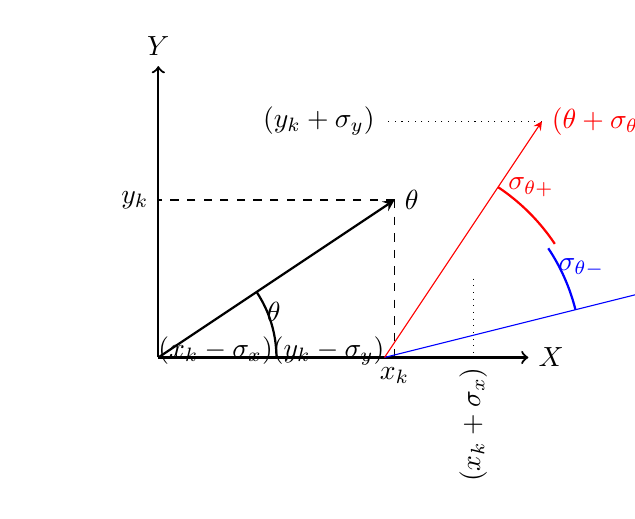
\begin{tikzpicture}
			\def \accX {3}
			\def \accY {2}
			\def \sigmaAccX {1}
			\def \sigmaAccY {1}
			\def \Xaxis {\accX+\sigmaAccX+0.7}
			\def \Yaxis {\accY+\sigmaAccY+0.7}
			%
			% Define angles
			% It is very important to get redundant parenthesis
			\pgfmathsetmacro{\bottomAngle}{atan(((\accY-\sigmaAccY)) / ((\accX+\sigmaAccX)))}
			\pgfmathsetmacro{\mediumAngle}{atan(((\accY)) / ((\accX)))}
			\pgfmathsetmacro{\upperAngle}{atan(((\accY+\sigmaAccY)) / ((\accX-\sigmaAccX)))}
			%
			% Draw coordinate system
			\draw[thick,->](0,0) -- (\Xaxis,0) node[right]{$X$};
			\draw[thick,->](0,0) -- (0,\Yaxis) node[above]{$Y$};
			%
			% Draw arrow medium position
			\draw[thick,-stealth](0,0) -- (\accX,\accY) node[right]{$\theta$};
			% Draw medium point
			\draw[dashed] (\accX,\accY) -- (\accX,0) node[below] {$x_k$};
			\draw[dashed] (\accX,\accY) -- (0,\accY) node[left] {$y_k$};
			% Draw angle
			\def \radiusMediumAngle {1.5}
			\draw[thick,black] ([shift=(0:\radiusMediumAngle)]0,0) arc (0:\mediumAngle:\radiusMediumAngle)node[below right]{$\theta$};
			\pause
			% Draw horizontal SD
			\draw[dotted] (\accX+\sigmaAccX,\accY-\sigmaAccY) -- (\accX+\sigmaAccX,0) node[rotate=90,left]{$(x_k+\sigma_x)$};
			
ode[rotate=90,left] at (\accX-\sigmaAccX,0) {$(x_k-\sigma_x)$};
			\pause
			% Draw vertical SD
			
ode[left] at (0,\accY-\sigmaAccY) {$(y_k-\sigma_y)$};
			\draw[dotted] (\accX-\sigmaAccX,\accY+\sigmaAccY) -- (0,\accY+\sigmaAccY) node[left]{$(y_k+\sigma_y)$};
			\pause		
			% Draw arrow bottom position
			\draw[-stealth,blue](0,0) -- (\accX+\sigmaAccX, \accY-\sigmaAccY) node[right]{$(\theta-\sigma_{\theta -})$};
			% Angle. Syntax: (startingPointX,startingPointY) arc (startAngle:stopAngle:radius)
			% ([shift=(t:r)] x, y) is the proper starting point, where (x,y) is the center and (t:r) is the polar coordinate of starting point.
			\def \radiusBottomAngle {2.5}
			\draw[thick,blue] ([shift=(\bottomAngle:\radiusBottomAngle)]0,0) arc (\bottomAngle:\mediumAngle:\radiusBottomAngle)node[below right]{$\sigma_{\theta -}$};
			\pause
			% Draw arrow upper position
			\draw[-stealth,red](0,0) -- (\accX-\sigmaAccX, \accY+\sigmaAccY) node[right]{$(\theta+\sigma_{\theta +})$};
			% Angle
			\def \radiusUpperAngle {2.6}
			\draw[thick,red] ([shift=(\mediumAngle:\radiusUpperAngle)]0,0) arc (\mediumAngle:\upperAngle:\radiusUpperAngle)node[right]{$\sigma_{\theta +}$};
			\end{tikzpicture}
		\end{figure}
		\onslide<6->{
			\begin{equation}
			(\theta_z - \sigma_{\theta -}) = \arctan \frac{y_k-\sigma_y}{x_k+\sigma_x}
			,\quad
			(\theta_z + \sigma_{\theta +}) = \arctan \frac{y_k+\sigma_y}{x_k-\sigma_x}
			\end{equation}}
		\onslide<7->{
			\begin{equation}\label{eq:sigmaPlusMinus}
			\sigma_k =(\sigma_{\theta +} + \sigma_{\theta -}) = \arctan \frac{y_k+\sigma_y}{x_k-\sigma_x} - \arctan \frac{y_k-\sigma_y}{x_k+\sigma_x}
			\end{equation}
		}
	\end{frame}
		
\end{document}